\documentclass[9pt]{article}
\usepackage[margin=0.45in]{geometry}
\setlength{\parindent}{0pt}
\usepackage[table]{xcolor}
\definecolor{tableShade}{gray}{0.95}
\usepackage[bottom]{footmisc}
\usepackage{amssymb}
\usepackage{url}
\usepackage{mathtools}
\usepackage{amsfonts}
\usepackage{booktabs}
\usepackage{graphicx}
\usepackage{tabularx}
\graphicspath{{./figs/}}
\usepackage{color}
\usepackage{float}
\usepackage[hidelinks]{hyperref}
\usepackage{siunitx}
%\usepackage[dvipsnames]{xcolor}
\usepackage{caption}
\captionsetup{font=footnotesize}
\usepackage[superscript,biblabel,nomove]{cite}
\usepackage{listings}
\usepackage[sharp]{easylist}
\usepackage{enumitem}
\lstset{breaklines=true}
\lstset{basicstyle=\fontsize{9}{10}\ttfamily, keywordstyle=\fontsize{9}{10}\rmfamily\bfseries}
\lstset{framesep=5pt}
\lstset{tabsize=4}
\lstset{numbers=left}

\lstset{xleftmargin=2em}
\usepackage{mathtools}
\bibliographystyle{unsrt}
\newenvironment{tightcenter}{%
	\setlength\topsep{2pt}%
	\setlength\parskip{3pt}%
	\par\centering}{\par\noindent\ignorespacesafterend}
\makeatletter
%\renewcommand{\@listI}{%
%	\leftmargin=25pt
%	\rightmargin=0pt
%	\labelsep=5pt
%	\labelwidth=20pt
%	\itemindent=0pt
%	\listparindent=0pt
%	\topsep=0pt plus 2pt minus 4pt
%	\partopsep=0pt plus 1pt minus 1pt
%	\parsep=0pt plus 1pt
%	\itemsep=\parsep}
\renewcommand{\@citess}[1]{\textsuperscript{\,[#1]}}


\makeatother


\begin{document}
	%\maketitle
	
	\begin{titlepage}
		\begin{center}
			\vspace*{1cm}
			
			\Huge
			\textbf{A-Level Programming Project}
			
			\vspace{0.5cm}
			\normalsize
			Raspberry Pi Facial Recognition Security System
			\vspace{1.5cm} \\
			\textbf{Dylan Callaghan}
			\vfill
			\vspace{0.8cm}
			\normalsize
			A-Level Project\\
			Candidate Number: 7005\\
			Centre Number: 40601
		\end{center}
	\end{titlepage}
\tableofcontents






\newpage
\section{Introduction}\label{sec_introduction}
My project is based around a facial recognition door security system using a Raspberry Pi 3B. This is a relatively inexpensive ARM based computer that is around the same size as a credit card and the same weight as a light mobile phone. This makes the Pi easy to mount in a case anywhere the security system may want to be used by the client. The security system works based on entering faces into a Python list-like data structure. The program will look for faces in a viewport from a Pi Camera, and using a file of trained faces, return the person that it predicts is in the viewport. I will be using a library such as the OpenCV library in python as a wraparound for the facial recognition portion of my project, along with many other libraries to make the project complete. The data for the faces can be entered at any time using a person stood physically at a camera and a dataset then being captured then and there. I will later add the functionality of a web interface to allow people to upload multiple photos of people from a mobile or desktop device, in addition to the option of them standing physically at the camera. This would be beneficial as it is not always possible to have a user on site at short notice, this allows the user to enter their facial data from anywhere. Once entered, the camera can be left in a constant ‘monitor mode’. ‘Monitor mode’ will scan the camera viewport for anything that resembles a face – if one is found , it will then be cross referenced to the data structure for faces that have been trained into the system. An unknown face will be picked up by the system if it was not a match to any in the database, returning an ID of 0 and a nametag of ‘Unknown’. In this case, a SMS message will be sent to a target mobile device using the Twilio API to inform the client of an unknown person at the camera. In ‘monitor mode’, the camera will also record to disk a snapshot of the viewing area of the stream at any time any unknown face is recognised, with overlays to display where the face is in the image – this is to keep records of intruders into the property for later use. As well as this, the user can choose to take a snapshot at any other time other than automatically if they wish. In order to comply with data protection laws surrounding the use of biometric data, the user will have to agree to a use-policy and privacy notice by using the device. For example, it is forbidden for a user to add biometric data for someone who has not given their express consent and it is the responsibility of the user to ensure they do not do this. That is the reason the physical facial enrolment is fundamentally a lot more compliant with data protection laws than the web upload option – it would be masses more difficult to get someone to enrol their face without their permission if they were not going to be stood at the door facing the camera. Unknown faces are not trained by the system, and the Haar Cascade will only detect them as a face without any other analysis on the data and treat them with complete anonymity. The web interface will be reasonably straightforward and not too advanced; a viewport for watching a live stream, buttons to perform actions such as training models or capturing data and downloading photos.

\section{Stakeholders}\label{sec_stakeholders}
My project is suited towards anyone over the age of 16 and/or a homeowner with the interest of their home security being close to their heart. It is probable that the user interface will require a small amount of technological literacy and it is true that it will not be fool proof. However, the GUI will make the program much easier to use its CLI counterpart – which daunts most novice users and would be described by many to be ‘not user friendly’. Most of the processing is done behind the scenes and the only operation is adding photos online, enrolling faces physically and downloading snapshots of the Viewport from the Pi. Although I am using the Twilio API myself, the end-user will NOT have to change any settings regarding the API, as it is my job as the account holder to ensure the code handles adding their own number to the system. The GUI and Web-Interface should be a fairly ‘plug and play’ experience, that is, to work from the get-go with limited hassle and a low level of learning needed. Despite this, any errors may still occur and there will be help on the web interface to assist users of any skill level with troubleshooting.

\section{Research into similar problems and their solutions}\label{sec_research}
A similar problem to mine would be the Ring™ doorbell system which connects to a Wi-Fi hotspot within a home and allows the homeowner to stream video from the doorbell at any time. The Ring™ doorbell also alerts the homeowner when someone is at the door. Whilst both these key ideas are vitally like my own, the Ring™ doorbell does not allow users to add people to a whitelist and it does not allow users to store footage locally – it must be kept on Amazon servers. As well as this, the relationship between Amazon and Law Enforcement services is not crystal clear so it is a grey area on how your data might be used – especially with (at least some of) the UK leaving the European Union which could allow for data protection and privacy laws to be overhauled to a large degree.  Whilst I fundamentally disagree with the use of facial recognition be it by the government or a large company, I would rather a small home user have the power to use it for their own good rather than the good of large multi-national corporations, the farming of data is now widespread across the whole globe  Even if you never ever use a service such as Facebook, in this day and age it is probable that they know who you are or have data on you at the very least. With that, my project will differ as it allows for centralised storage of recorded and cached footage that can be modified at any time by the user, kept on a device within the LAN of the router and firewalled to prevent outside contact. My project will also have to comply with data protection laws surrounding  biometric data in order to keep the user(s) of the product safe just as any system using biometric data must comply with data protection laws.
Another product with a similar theme to mine is the Nest Hello doorbell offered by google. This is again like the Ring™ doorbell with live streaming of a camera and the offer of continuous recording. Another similarity is the storage on the cloud as opposed to local storage – leaving the end-user with less control over their data. It is especially with the biometric and other sensitive data types that I would like complete control over how my data is used and how the data of other people who consent to using the product is used. Unlike the Ring™ though, the Nest Hello doorbell must be a wired connection – a feature that could make installation harder.  \\
Finally a product that is very similar to mine can be seen in this article by Techradar. This solution uses MotioneyeOS in order to stream video from the Raspberry Pi camera to a webpage accessible by devices on the network via the browser. There is a reasonably simple control panel for controlling settings and configuring devices. Rather handily, there is an option to upload recorded files straight to many popular cloud storage services such as Google Drive and Dropbox, something I may consider adding in the future as it is very convenient for the end user.
Many doorbell-based security products require a subscription service of some sort in order to access all the features of the security system. This means that the price you pay for the product is not the final price and many people likely will not know this until they have purchased the product. \\
I hope to take the best from these existing similar projects and improve on places where they have perhaps fallen short. Some things, such as battery connectivity, may be a little too far-fetched for my limited budget though – these are not affected by code however, and could easily be added at any point of the project. Unlike both the Ring™ and the Nest Hello doorbells, I will ensure all files such as captured images stay local and free for the end-user. There will be no cloud subscription plans and the price paid for the product is the final price, all the features available will be usable as soon as it is installed, no extra fees.

\section{Essential features necessary for a computational solution}\label{sec_essential}
Firstly, my program will have to allow the input and output of a video stream from a Raspberry Pi NoIR camera in order to be analysed with the library of some sorts, likely OpenCV. This is like the other products shown above which all handle an incoming video stream from a built-in hardware camera. The main data coming through the system will be the data from the video stream. This is handled by the python software layer and interpreted as needed. There will also be some user input over the web interface using a keyboard and mouse – allowing the end user to control the system from their own device. This data will be passed over the internet and straight to the Flask webserver on the Pi, where it is then interpreted to perform actions as my code requires.

\section{Limitations of my solution}\label{sec_limitations}
The main limitation of my solution will be my inexperience using facial recognition and AI / Machine Learning as a whole. Despite researching this extensively beforehand, I have limited practical experience and I strongly suspect there to be many errors along the way during the coding and practical building of my project. I will combat this by writing each important section of the code as separate files (which will form a library of sorts) to ensure that basic building blocks of my code can be completed and left intact without any errors from changing other sections of the code. These can then be put back together in a final runtime file to be used 24/7. Strong and vigorous testing and debugging procedures at extremely frequent intervals will ensure I do not venture too far from the last stable state of my project and if anything becomes too ambitious, I may have to find an alternative solution or move on from the idea altogether. GitHub will allow me to see past versions of my project very easily – different branches can be made for different features and issues can be made and attached to features, closed by a pull request. This workflow will allow me to go through the project with an absolute stability and ensure that any errors are never permanent. I believe that using GitHub will allow me to experience more of a real-world workflow, despite me being the only contributor. Version control and bug management are key things that coders must control whether by themselves or in a team. GitHub is great for this as it uses the push/pull commit system which is great for version control – if I ever find that I have stepped too far with my new code I can always easily reset to an earlier version, without having hundreds of differently named files of different versions (namely things such as ‘asdfghjkl.py’ which I find myself to hoard often)
The next limitation is time. There are certain things that are beyond my control such as waiting for programs to compile and other such things. Installing and compiling programs might end up taking a significant portion of time out of writing code and testing my project to ensure it is of a high standard. The only way I can think to combat this is to try and multitask at an extremely efficient level – moving on to other parts whilst waiting for others to complete or finish a task. As well as this, I will have to be extensively reading documentation and debugging instead of moving forward with new features and general progress. I have less than a year to complete a project that is on a totally different level to what I have done previously. I do not wish to rush any code and ensure that it is both completed in the time-frame given, and to a very high standard. If my project does not meet all the success criteria outlined later, I will personally consider it a complete failure.
The project requires some sort of graphical front-end which will be in the form of a web-interface in my project. I currently have 0 experience in web development and linking this to my python code that will be executed at runtime. Despite researching beforehand, this somewhat ‘side’ portion of my project could potentially be the hardest part for me personally despite it being somewhat simple for others. I hope that reading documentation and debugging errors will be enough for me to move forward and complete the web-facing portion of my project in a reasonable amount of time whilst still maintaining a reasonable amount of quality. Even if the base code works and can be executed through a CLI on the Raspberry Pi directly, without a GUI, my project might be void. It will therefore be difficult to complete the web-facing side of the project whilst still focusing enough on the bulk that goes on behind the scenes processing and performing operations in order to create a working facial recognition security system.
The camera in my project is the Pi Noir Camera that operates in low light / dark conditions using infrared. If there is no IR source in the room or outside area however, the image returned will be either extremely broken and grainy or just plain black – a failure of the key feature of my system. Furthermore, the way in which faces are recognised is going to be with ‘Haar Cascades’ which I will discuss later in this coursework document. Whilst being a very popular way to recognise objects such as faces; it is also known to give false readings in the forms of both false positives and false negatives. It is unlikely that the end-user will have a vast library of photos of each user to be added to the system. And it is unlikely that every user will want to enrol their face in different weather conditions and different times of day in order to get more confident readings (regardless of if they are positive or negative). For this reason, the user may receive too many annoying messages of false positives and move away from my product. It will be difficult to find the correct balance between speed and accuracy.
Finally, the use of a camera and the raw computational power required to record video, stream video, analyse each frame for a human candidate and train faces means that CPU and RAM / DISK usage will be very high. Even at idle load, my Raspberry Pi runs at an abnormally high temperature possibly due to a manufacturing defect. It is possible that my Pi may throttle and have significantly reduced performance, it might even break altogether. Both situations would render my project to be broken and unsuitable for the end-user (and therefore a fail altogether). Not only this but the Pi will need a quality power supply, and the placement of the camera may be tethered by the length and fidelity of the power supply – resulting in less than convenient positions available for the camera to operate in. This is why a battery may be a much better choice – however my budget does not allow for that luxury and the power supply will need to be hard-wired into the wall or a cable ran to an extension lead near the placement of the product.

\section{Minimum Required Hardware and Software configuration}\label{sec_hardware}
\textbf{Storage} -- 32GB or greater, the reason for this size is to allow both the installation of the operating system and the ability to save lots of snapshots onto the disk.\\\\
\textbf{CPU} -- 2 Core 1GHz CPU with graphics support. The reason for this is that OpenCV is CPU heavy and without a decent CPU, the processing may grind to a halt or even hang.\\\\
\textbf{RAM} -- 1GB DDR2 RAM. The processing is also RAM heavy, without enough RAM (or a swap file) the system may crash. \\\\
\textbf{Network} -- Ethernet connectivity or 2.4GHz wireless to allow for the webserver to work (and for me to connect to the Pi to code headlessly).
I have owned a Pi 3 for a while and this is what I will be using for the project, despite a Pi 4 being a better candidate. The Pi Zero offers a small form factor which may be better for a discrete camera, but it lacks the processing power for OpenCV. I will be using PuTTY to SSH into the Pi for the initial setup and then moving onto a VNC server to allow me to access the Pi from my standard desktop PC. I think that this will be easier than hot swapping keyboards and mice and changing inputs on my monitor 24/7. \\\\
As well as this, we will also need\\\\
\textbf{Power Supply} -- 5V @ 2.4A to provide the Pi with enough power to run without throttling doe to undervolting, and also to power the NoIR.\\\\
\textbf{Cables} -- We need enough cables to connect everything together. Figure \ref{fig_raspberryCables} shows the cables needed between each component. The NoIR comes with a ribbon cable
\begin{figure}[H]
	\centering
	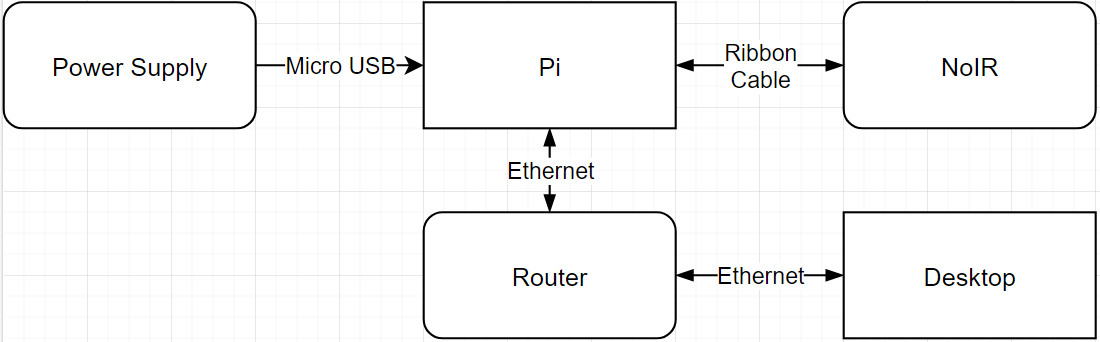
\includegraphics[width=5in]{raspberryCables.png}
	\caption{A diagram that shows the connections between components and the respective cables}\label{fig_raspberryCables}
\end{figure}

\newpage
\section{Success Criteria}\label{sec_succes}

\begin{small}
	\subsection{Success Criteria for the device setup}\label{sec_device}
	\begin{enumerate}
	\setlength{\itemsep}{4pt}
	\setlength{\parskip}{0pt}
	\item \textbf{Ensure that the Pi is enabled for SSH connection from my desktop computer.}\\
		This should be connectable via the local IP address of the Pi from any computer on the network. This allows me to remotely connect and code from my desktop computer – making the development process much easier.
	\item \textbf{Set up the VNC server on the Pi and allow connection from my desktop.}\\
		This provides similar functionality to the SSH connection capability as above – allowing me a better development experience. This should be at least a 768p desktop for a balance of screen space and speed.
	\item \textbf{Set up the NoIR camera with the Raspberry Pi using \texttt{raspi-config}.}\\
		This can be verified as working using the \texttt{raspistill} command in the terminal, a still photo should be taken. The orientation is irrelevant as this can be configured later on in the python solution.
	\item \textbf{Change the swap size to allow for a greater memory capacity.}\\
		There is a possibility that the solution uses more memory than available. This ensures me that there will be a sufficient amount of memory at the negative of wearing out the SD card storage at a quicker rate. This is because flash memory used in SD cards has limited read/write cycles before data starts to rot and become corrupt. I think a swap size of 2GB would be a good amount.
	\item \textbf{Ensure that the latest version of Python 3 is installed (that is compatible with OpenCV) along with needed modules such as pip.}\\
		This is to ensure that I will be able to code the solution and not have to spend time finding and installing libraries when I could be developing the solution. This is verifiable by typing python in the terminal and noting the version installed. 
	\item \textbf{Acquire the latest versions of libraries with the pip command in the terminal. Similarly, pip list will show everything that has been installed by pip – a checklist can be used to check off that libraries have been installed.}
	\end{enumerate}
\end{small}
\begin{small}
	\subsection{Success Criteria to ensure the enforcement of chosen programming constructs}\label{sec_program}
	\begin{enumerate}
		\setlength{\itemsep}{4pt}
		\setlength{\parskip}{0pt}
		\item \textbf{Prefix variable names with important information to make the code more readable.} \\
		Taking the time to prefix information such as datatype or what the use of a variable is makes the code easier to read. Not only this, but if the code needs to be debugged then it is easier to understand what the purpose of each variable is as it is already there in the name. Whilst not the primary function, a helpful side effect is that the auto-completion offered by the IDE may work more efficiently; when you know you are going to be using a variable that is a number, typing `int\_’ will return the auto-complete list that contains all integer variables – the coder will not have to search through the code for the correct variable name. It is likely that I will follow the naming convention as below:
		\\\centerline{\{datatype\}\_\{variableName\}}
		This is a combination between Hungarian notation and switch (camel) case, two very popular programming standards. The camel case makes the stem part of the variable name easier to read by marking different words by using a capital letter. An example of a real variable is as follows.
		\\\centerline{obj\_faceRecogniser}
		\item \textbf{Add detailed comments to code} \\
		Comments allow other people to read your code and still understand what is going on, even if they would code a solution to the problem in a different way – they explain how the code works which is especially useful for when the purpose of the code isn’t amazingly clear. For me, this will allow me to return to previous code and understand what my thought process was whilst making that piece of code, even if I had forgot. Yet again, this will also make debugging easier as the comments can allow the programmer (me) to see if there are any logical incompatibilities in the code at a quicker glance than working through the actual code line by line to see what happens with the variables.
		\item \textbf{Use GitHub for version control} \\
		GitHub as a platform allows me to commit edits to code and ensure that they are well documented. Each feature can have its own branch that is merged back to the main branch once the feature is fully complete. This ensures broken code is not added back to the production level source code. Each commit has bug tracking and I can choose to fallback to different versions of code if I have overstepped and broken the code to an unrecoverable level. I think it is realistic to be using version control such as GitHub as it is very common to find this system being used in program production houses.
		\item \textbf{Ensure code is modular} \\
		To provide a better development experience, code should be as modular as possible. Each module can have its own development cycle and ensure that the building blocks are well complete before moving on. This is preferable to me as opposed to a linear code process as it deals with smaller chunks of code when debugging and prototyping. I think that for me, focusing on small bits at a time 
	\end{enumerate}
\end{small}
\newpage
\begin{small}
	\subsection{Success Criteria for the solution}\label{success}
	\begin{enumerate}
		\setlength{\itemsep}{4pt}
		\setlength{\parskip}{0pt}
		\item \textbf{Gather an incoming camera stream from the Pi Camera in python.}
		\begin{enumerate}
			\item \textbf{Is the view of the camera clear and is it orientated correctly? It should be the standard way up and look clear.}\\
				This is important as it will ensure the feed will be working properly for later sections of the project, if it works now and fails later then we know it is something recent that broke during that stage of coding as opposed to this crucial early step. Setting this up correctly now ensures that the code later during the rest of the project will be able to rely on this fundamental code. A bad way to code would be to rush straight in and try to code the whole thing at once, making it much harder to debug and identify and solve as there is so many more potential failures.
			\item \textbf{Is there any lag, how much? Are there framerate drops? Does it adversely affect performance?}\\
				This is important as it is preferred to have a smooth video to easily see what is going on. Choppy video negates the positives of a camera monitoring an area, as we may not even be able to see the actions of people through the camera very clearly. Additionally, input lag would make the experience for anyone watching the online stream less enjoyable – in extreme cases, the stream may not at all accurately represent what is going on in front of the camera. This would make the promised ‘live streaming’ aspect a lie and make the solution void. I aim to have an average of at least 5fps over the course of a 2-hour test run.
		\end{enumerate}
		
		\item \textbf{Use a machine learning library to identify objects that look like faces and draw a bounding box (or multiple) around the identified face(s).}
		\begin{enumerate}
			\item \textbf{Is the box clear to see? It should be at least 2 to 3 pixels thick at source.} \\
				This is important as the feed will later be able to be viewed on a smartphone with a smaller screen. It is essential that the box is clear so it can still be seen around any objects in a frame – even on a mobile device. It should be at least 2 to 3 pixels thick on the source frame, before any post-resizing on other devices. I would say that the bounding boxes that identify faces are a fundamental part of this project – they show the end user that the solution is, indeed, identifying faces in a frame.
			\item \textbf{Does it identify faces well? Are there any false positives or negatives?} \\
				Both false positives and false negatives will impact the accuracy of my solution and make it a less viable product in general. I hope to especially reduce the rate of false positives of unknown people (which will send annoying texts to the user through Twilio on the condition of repeated false positives). There are various parameters that can be tweaked in order to change how many machine learning libraries identify faces, and the accuracy at which this happens. I hope to perform tests to find which sets of parameters yield the most accurate result. I hope for around 75\% accuracy with a database of 5 qualified people.
		\end{enumerate}
		
		\item \textbf{Add code that can take photos of the Pi Camera viewport to be used in the collection of a dataset. Crop from facial bounding box.}
		\begin{enumerate}
			\item \textbf{Do the photos crop correctly to the bounding box?}\\
				It is important that the photos saved are only of the faces and not of other objects that are present in the frame, this is so the trainer has the correct data to train the recogniser. The photos should be cropped square and the face should be centred in the crop
			\item \textbf{Are the saved photos the correct object (the face in the viewport)?}\\
				This is important especially for the trainer step later. The dataset needs to be coherent for the trainer to coherently and accurately know what unique properties ton look for in an object to match to a person. The more people added to a dataset that they should not be in, the more chance that the trained recogniser will recognise too many people as the same person – a failure. It is important that each unique face has a different ID so that the trainer separates different faces.
		\item \textbf{Does the code save enough photos?}\\
				This is something that can and will be down to me to decide. The trainer needs enough photos with enough variation in order to accurately know what to look out for in different faces. Despite this, there are going to be space limitations – especially if many people are added to the system. I will have to find a good balance between having enough photos for accuracy whilst keeping the size on disk low.
		\item \textbf{Are the files named correctly so that they can later be read and parsed by the training code?}\\
				The naming scheme of the files need to follow a specific format for the trainer to match different people’s photos together with the same ID, and form collections of the same person. It is also required that each file has a unique name. This will likely be in the format:
				\begin{tightcenter}
					{"\{ID\}.\{Num\}.jpg"}
				\end{tightcenter}
				This is simple enough to be read by the trainer function whilst keeping the functionality necessary for the function to work which is a good compromise. It is likely that there could be 100s of different photos with many different people.
		\end{enumerate}
		
		\item \textbf{Add code that trains the dataset gathered into a file which can be read by the machine learning library in order to then detect registered faces in the viewport. This will use an ID system obtained from the images.}
		\begin{enumerate}
			\item \textbf{Can the code read the files in the dataset and use a trainer function correctly?}\\
				The code needs to be able to recognise the naming scheme of the dataset files in order to then train the photos to be recognised by a recogniser function. It is important that all files are read properly so that the trained file is the most accurate that it can be. The trainer function should output a single file which can be used by a recogniser – a function that scans the viewport for trained faces.
			\item \textbf{Does the trainer file save successfully?}\\
				If the file does not save, no recognition can take place as the recogniser will not have anything to work with.
		\end{enumerate}

		\item \textbf{Add code that uses the trainer file to then recognise faces in the viewport}
		\begin{enumerate}
			\item \textbf{Can the recogniser read the trainer file?}\\
				The recogniser needs to be configured to read the trainer file, and then scan the viewport for faces that match any faces in the trained file. This forms the basis of the identification part of the recognition system.
			\item \textbf{Is the accuracy of the recogniser great enough to be pushed to production?}\\
				It is important that the recogniser can detect whose face belongs to who with reasonable accuracy, failure to do so will result in an incoherent security system that could potentially not function correctly at all – allowing intruders to gain access without much notice.
			\item \textbf{Can it recognise more than one face?}\\
				There will often be situations in which there is more than one face in the viewport. It is therefore required that the recogniser can scan a viewport that contains more than one face and work out the ID of each face present accordingly, this is to prevent people from possibly fooling the system by placing a printed known face and placing Infront of the camera whilst moving past undetected themselves.
			\item \textbf{Can it return the correct IDs even in extreme circumstance?}\\
				Can the recogniser return correct IDs on people that look extremely similar? Probably not and I do not expect this part of the success criteria to be passed in my opinion. I do not think the Raspberry Pi has the computing power necessary in order to run at a quality high enough to detect such small differences in appearance.
			\item \textbf{Does it allow for returning ‘unknown’ for an object that resembles a face but is not registered?}\\
				This is important especially for the stage that will incorporate Twilio API into my python code. The recogniser must account for any faces that are seen that are not trained to be recognised. These should be marked as ‘unknown’. This will allow a Twilio subroutine to then send a text to the user and inform them of the date, the number of unknown faces and hopefully also send a photo of the frame at that specific moment.
		\end{enumerate}
		
		\item \textbf{Add code that starts a webserver in python (This will almost certainly be done with the Flask library)}
		\begin{enumerate}
			\item \textbf{Does the webserver run locally, and can it be accessed on the house intranet using a different device?}\\
				The webserver needs to be accessed by devices on the same network before thinking about expanding to the whole internet using port forwarding. The webserver is what will allow the end-user to access the video stream and control the software so without this working correctly, the project fails.
			\item \textbf{Can the webserver display HTML pages with CSS?}\\
				In order to add buttons and other various functions, I need to be able to display HTML pages with CSS. The CSS will be simple but will allow me to make the buttons look just a little bit nicer than before and ensure that the user interface is of a standard that even a novice user could understand. In the event that I finish my solution earlier than expected, I should also add a toggle to enable advanced settings for very experienced users.
		\end{enumerate}
		
		\item \textbf{Transfer the previous camera-based code over to the webserver code.}
		\begin{enumerate}
			\item \textbf{Can both sets of code still be called?}\\
				I need to make sure that I did not create any conflicts by merging these wo sets of code together – even if it doesn’t look like it at the surface it may impede performance and usability later down the line if I do not thoroughly check the code. I should also check for any forms of spaghetti code and remove these as required, keeping the source code as optimised and easy to read as possible.
		\end{enumerate}
		
		\item \textbf{Add a page to the website that livestreams the video feed from the camera after machine analysis using the selected library.}
		\begin{enumerate}
			\item \textbf{Is the quality of video good?}\\
				The quality of video needs to be good enough to be used to identify details of any unknown people caught by the software in a still image. If the image is broken, blurry or has any other artifacts, the project will have no benefit at all in comparison to a normal, cheap CCTV camera from a cheap electronics store. The Pi NoIR camera has a decent resolution so any reduced quality will likely be from my process of handling the image data.
			\item \textbf{Can this be viewed on other devices?}\\
				I do not know what device the end user will choose to view the web-interface on – so it is important that I create the website so that it can be viewed on many types of device with many different display configurations. There are many such factors similar to this that a programmer must consider when writing a solution. This is probably one of the more basic considerations when making a website but any further important considerations that I find can be added when I perform testing later on in the development stage.
			\item \textbf{Can it be viewed on more than one device at once?}\\
				In the situation that there is more than one person living at a house (which will be common). It is important that more than one device can read the video stream on the website at once in case multiple members of the household would like to view the stream. This may sound simple, but I expect to run into threading and file locking issues due to the nature of how I am going to serve the frames to the webserver. The code should allow the stream to be viewed by more than one device with ease.
			\item \textbf{Can the frame caught still be used by other parts of the code whilst it is being streamed?}\\
				This relates to the threading and locking issues I described above. I aim to have a universal frame that can be used by many sections of the code such as image saving and the web-interface. This should be updated at least at 10 frames per second to avoid the video seeming too jittery. However, all functions that require the frame must finish their job before the frame changes, this will add a small amount of lag but most importantly will require the use of a thread and lock system which can be done with a number of libraries on Python. The threading and locking system also ensure that only one thread is accessing the camera at once.
		\end{enumerate}
		
		\item \textbf{Add code that allows the user to take screenshots of the current frame and save them to the device.}
		\begin{enumerate}
			\item \textbf{Choose an appropriate file format}\\
				It is important to balance both quality and file size. I think that a high-quality JPEG is probably the best way to save screenshots due to the fact that the compression is not noticeable to most people, and the file sizes are smaller due to the lossy compression involved.
			\item \textbf{Does the file have an appropriate name?}\\
				This is important as the file needs to have information both in the name and the metadata to accurately describe the context of the photo. Whilst metadata can usually do the job of containing this information, many users (especially novice users) may not be able to access this important data. Due to this, most of the important context will be held in the filename such as the date and time that the photo was taken. I expect the format to be something resembling the following.
				\begin{tightcenter}
					{\{YY\_MM\_DD\}\_\_\{HH\_MM\}.jpg}
				\end{tightcenter}
		\end{enumerate}
		
		\item \textbf{Add code that allows users to upload their own photos to add to the dataset, without having to stand in front of the camera}
		\begin{enumerate}
			\item \textbf{This should be presented as a button on the website, which then takes the user to the accompanying system upload dialogue.}\\
				I am doing it as a button as this is already a very common way to solicit user interaction within a webpage – it is extremely common that a user has pressed buttons in order to interact with webpages
			\item \textbf{Does the webserver allow the user to upload multiple images at once?}\\
				One picture is nowhere near enough data for a trainer to accurately learn about facial features and uploading one photo at a time would be a very tedious process. 
			\item \textbf{Does the solution handle cropping the photos and adding to the dataset correctly?}\\
				The solution would need to crop the photos so that other unnecessary data is not included.
		\end{enumerate}
		
		\item \textbf{Ensure that the quality of the web-server (once all elements are added) is good enough}
		\begin{enumerate}
			\item \textbf{The page should adapt to different screen sizes and be responsive}\\
				This is due to the fact that the page is likely to not only be viewed on a desktop, but a mobile phone also. The aspect ratio of phones is more similar to the inverse of the aspect ratio of monitors. Therefore, if the style of the webpage is hard coded to the display size and ratio of a monitor, it will not look correct on a phone. Responsive (adaptive) design overcomes this problem, by allowing the format of the webpage to change depending on the device that it is viewed on. As a result, the webpage can look different on a mobile phone when compared to the desktop version. If needed, other devices can be added also (although I will only be adding true functionality to phones and desktops)
			\item \textbf{The buttons should be clearly annotated}
				Buttons should all have labels, so the user knows the purpose of each of them. If the delete button is only red with no text, the user may get the idea of the negative impact, but they will not know exactly what it will be. Therefore, the buttons should be styled with elements such as text, colour, and more. This makes it perfectly clear to the end user. 
			\item \textbf{Clarity is important; the function of all elements should be obvious even for a novice user}\\
				The user may be experienced with computers, or not very competent at all. It is important that the full functionality is laid out at clear as possible with as little instructions needed. Users do not like reading through pages of extensive documentation only trying to find a small and easy use-case relevant for them. For this reason, the webpage should be laid out in such a way that the functionality is intuitive – that is, the user does not need to read too much in order to understand how to use the controls on the page
		\end{enumerate}
	\end{enumerate}
\end{small}
I can refer back to this success criteria during the iterative development process to ensure that I have completed all the parts of the solution that are necessary. The large amount of detail in this success criteria means that I will be able to have a solid base to construct my solution on. Each point adds culminates to provide a framework for the construction of the final solution.\\\\
References to each group of success criteria will be with the symbols $\alpha,\beta,\gamma$ respectively (in order of appearance)
\newpage
\section{Design of the solution}\label{sec_design}
\subsection{Decomposition of the problem and application to the solution}\label{sec_decomposition}
\subsubsection{The non-web areas of the solution}\label{sec_nonWeb}
In this section, I will be breaking down the solution into multiple sections which are suitable for a computational approach. The code here is mostly of a pseudocode format, although it will be very `pythonesque’ – with many keywords matching that of Python.
As a whole, the non-web facing portion can be represented by the flowchart on Figure \ref{fig_flowOverview} – this part shows the logic of how all face-related functions works.
\begin{figure}[H]
	\centering
	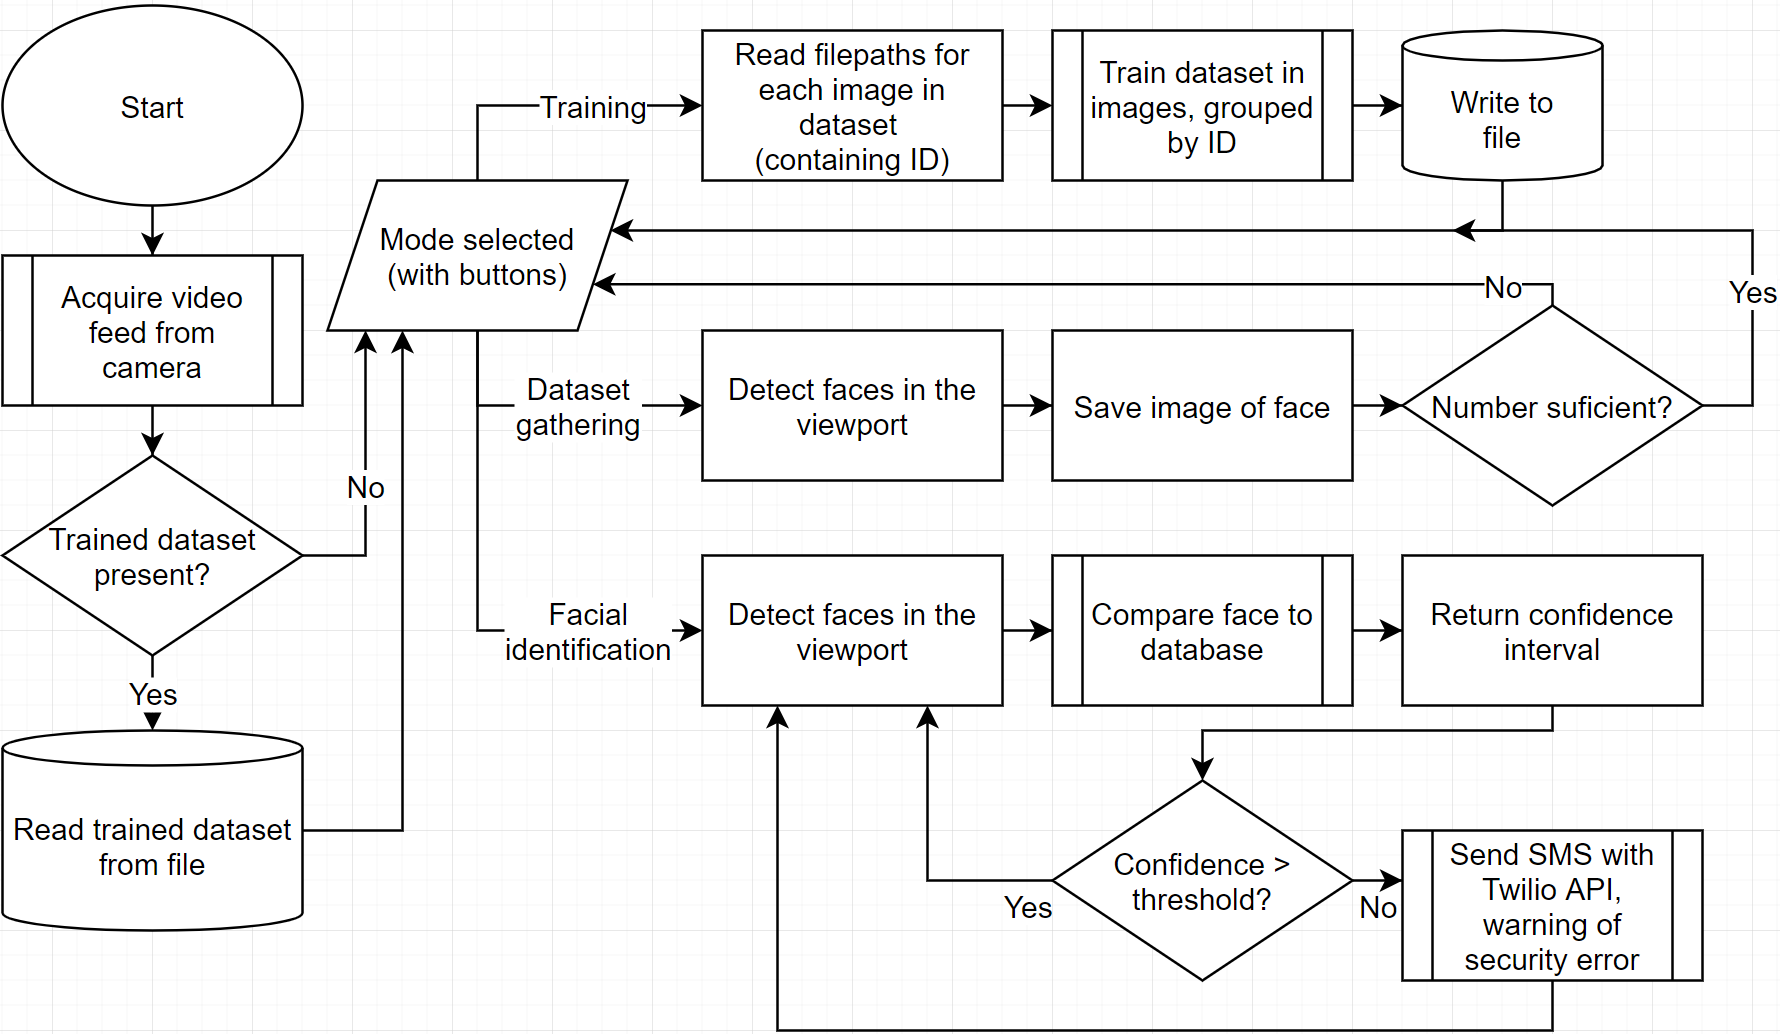
\includegraphics{flowOverview.png}
	\caption{Flowchart showing the logic behind the non-web section of the solution}\label{fig_flowOverview}
\end{figure}
We can go more in depth into many areas of this flowchart. This shows decomposition and abstraction at work heavily – we are breaking the problem down and then removing all unnecessary parts that the solution does not require in order to function correctly and follow the logic that is intended. 
Firstly, the solution will need to acquire a camera feed from the NoIR camera. In the event that there is no feed, the solution should warn the user and on the web interface, prompt for a restart. This is the first and most important step as every other part of the solution requires the presence of a video feed from a camera. In Python, I imagine that I will be using the \texttt{try ... except ...} syntax. The first part allows me to specify what happens in the case that the camera feed is working, with the except loop being for the case that the camera feed does not work (or that the camera feed abruptly stops without user input).
So, the pseudocode implementation would be something similar to the following, along with the flowchart diagram underneath.

\begin{lstlisting}
try:
	assert cameraFeed {is_working} == True
	...
except AssertionError:
	display errorMessage
	display restartPrompt
\end{lstlisting}
\begin{figure}[H]
	\centering
	\includegraphics{flowCameraworking.png}
	\caption{Flowchart that shows the try and except syntax for the camera validation}\label{fig_cameraWorking}
\end{figure}
This code, despite being rather simple, is fundamental to the solution as the other blocks of code all rely on a working camera feed. In the event that this is not possible, it is important to have a good fallback subroutine that still gives the end user lots of options. This is because the end user will not have access to the source code, and they likely are a novice computer user – they therefore both lack the skill and the tools required to debug the code and fix it themselves. As with most of the following sections, it is important to code for as many possibilities as possible, so that the end user encounters the least amount of unintended errors as possible.\\\\
The next stage relies on a library that can handle computer vision processing or similar features. For this purpose, I have chosen the python implementation of OpenCV. 
Directly from the website, ``OpenCV was built to provide a common infrastructure for computer vision applications and to accelerate the use of machine perception in the commercial products. Being a BSD-licensed product, OpenCV makes it easy for businesses to utilize and modify the code \cite{openCvAbout}”. The reason I have chosen this is due to the fact that it is not only a well-made library, but the documentation is immense and covers all areas in great detail. Absolutely everything I need to harness the functionality of this library can be obtained directly from the documentation which means I can spend less time learning to use the library, and more time coding a solution with the library. Despite making this choice, there are many more sub-choices within OpenCV which I will cover later in the relevant sections.
The next stage is taking the camera feed and beginning to recognise faces within the feed. Any additional processing comes under its own subroutine in this case, and the face recogniser acts as a core functionality once again. For the face detection, I will be using a Haar based cascade classifier – this uses a series of positive and negative images in order to train a classifier (the object used to differentiate between faces and non-faces). For the purpose of saving time, I will be using a pre-trained face detection classifier that has been produced with a Haar-based methodology. Despite this, I do not think that this choice reduces the complexity of my solution due to the fact that the implementation of this Haar cascade is extremely similar to how the classifier would have been constructed regardless. Therefore, if I can correctly show an implementation of the Haar cascade in context of face detection and identification, I am also showing that I could construct the Haar cascade anyway – as the methodology is much the same.
\begin{figure}[H]
	\centering
	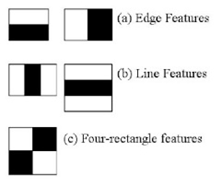
\includegraphics{haarCascades.png}
	\caption{Types of features detected by Haar Cascades \cite{haarImage}}\label{fig_haar}
\end{figure}
“A Haar feature considers adjacent rectangular regions at a specific location in a detection window, sums up the pixel intensities in each region and calculates the difference between these sums \cite{haarInformation}”. Due to this, the resolution of the incoming stream needs to be high enough in order to preserve fine details that will help the Haar cascade to classify a face. I will need to keep this in mind later when deciding the parameters for the incoming stream. The diagram on the right shows the sorts of features that a Haar cascade can detect; there are often tens of thousands of such features in one picture, and the datasets needed to construct a Haar cascade classifier from scratch are rather large, larger than the datasets needed to recognise faces at least.
The pseudocode for face detection will be something resembling the following (there are also OpenCV keywords included here).
\begin{lstlisting}
set faceCascade = {path_to_cascade_xml} 
set stream = videoFeed from {device}
set stream{height} = height
set stream{width} = width
while True:
	set gray = stream{convert_to_greyscale}
	set faces = detect faces in stream with {parameters}
	for each face in faces:
		{draw_boundingBox} around face
release videoFeed from {device}
\end{lstlisting}
Despite being rather simplistic as a result of abstraction in the pseudocode, this code will load a cascade from a file, initialise incoming video feed and then convert the stream to greyscale. The reason for this is due to the fact that abstraction is a theme that runs throughout the core of my entire project -- removing parameters that are not needed for the detection of faces such as colour is a prime example of abstraction at work. \\
The most important thing for Haar cascades are the edges of materials in the image, and colour is irrelevant (therefore removed). The solution will then detect the faces within the grayscale image and draw a bounding box around each detected face for identification. The parameters used for this are library specific and will be discussed during the iterative development phase. As previously discussed however, the choice for the parameters is rather important for the final working functionality of the solution. 
The next stage comes from adding the ability to create a dataset from a face that is in current view of the NoIR camera. This is nearly as simple as appending a few extra details to the previous pseudocode, as much of the underlying logic is fundamentally the same. As mentioned previously as apart of the iterative development methodology, I would prefer to code this linearly and iteratively before then adapting it to an object-orientated solution if I get the chance.
\begin{lstlisting}
set faceCascade = {path_to_cascade_xml} 
set stream = videoFeed from {device}
set stream{height} = height
set stream{width} = width
set ID = numericUserInput(idOfPerson)
set_iterations_left = numericUserInput(numberOfPhotos)
while iterations_left > 0:
	set gray = stream{convert_to_greyscale}
	set faces = detect faces in gray with {parameters}
	for each face in faces:
		{draw_boundingBox} around face
		write {image_of_gray_face} to {device} with {filename}
		iterations_left -= 1
release videoFeed from {device}
\end{lstlisting}
We can see the new lines in this code; the first new lines allow the user to input a numeric ID for the face they wish to add to the dataset. The next line sets an iteration number as defined by another numeric user input – this number in context of this code snippet relates to the number of photos that will be saved to the device of that ID. This can be changed at a per-ID level and allows for more detailed datasets of different people. \\\\
The next part of the solution is taking the datasets of faces that we have grabbed using the first section of code then constructing a trained dataset from them.  This trained dataset is much like a database holding instructions to identify faces that will later be used to identify individual facial features. I am going to be using an LBPH-based feature recognizer. An example of the way in which this recognises features from images is shown on Figure \ref{fig_LBPH}
\begin{figure}[H]
	\centering
	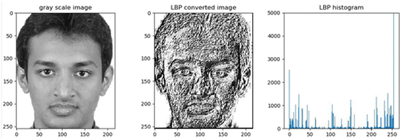
\includegraphics{lbphRecognition.png}
	\caption{A picture showing each stage of the LPBH recognition process \cite{lbphDiagram}}\label{fig_LBPH}
\end{figure}
This looks somewhat similar to the Haar based system. A simplified way of describing it would be that it converts an image to grayscale, splits the image into smaller 3x3 sections and then performs operations such as edge detection and more on each of those sections. The resulting middle image on Figure 6 shows the result of this LBP process. This middle image shows the features of the face in the first image. A histogram showing the number of similar LBP values in a region can be constructed and is shown on the right. This histogram describes that unique face as it can be perceived as a ‘fingerprint’ of sorts. As a result, we can identify faces from one another by comparing their LBP histograms. A table of the advantages of this algorithm are shown below.

\begin{table}[H]
	\centering
	\begin{tabular}{@{}p{3in}p{3in}@{}}
		\multicolumn{1}{c}{\textbf{Advantages}}                        & \multicolumn{1}{c}{\textbf{Disadvantages}}        \\ \midrule
		Computation is simple with only a few stages                   & Rotation of face affects result                   \\
		Good performance even on low-powered devices due to simplicity & Size of database affects accuracy                 \\
		Does not rely on colour                                        & Complexity   increases non-linear with image size \\ \bottomrule
	\end{tabular}
	\caption{A table showing the advantages and disadvantages of the LBPH algorithm}
	\label{tab_lbphProCons}
\end{table}
The pseudocode for the logic implementing this algorithm will be something resembling the following.

\begin{lstlisting}
set datasetPath = {path_to_dataset} 
set recogniser = {LBPH_recognizer_cv2}
set faceCascade = {path_to_cascade_xml} 
def findImagesIDs(datasetPath): 
	set imagePaths = {list_of_paths_to_images}
	set ids = [] 
	set faces_array = [] 
	for path in imagePaths: 
		set imgGray = {convert {image_at_path} to grayscale}
		set imgBin = {imgGray as binary}
		set faces = {find_faces} with faceCascade 
		for each face in faces:
			faces_array.append(imgBin of face) 
			ids.append(ID) 
	return faces_array, ids, imagePaths 
set faces, ids, paths = findImagesIDs(datasetPath)
{train recognizer} with (faces, ids) 
{write trained recognizer} at {path_to_trained_dataset}
\end{lstlisting}

We can see that this code is much different than previously – this is since there is no input feed here as this part of the solution just uses the files already taken from the dataset constructed in the previous section of the code.
The first step of the process are some initialisations such as the path where the images are saved; other things such as the path to the face cascade are needed also. We must also create a recogniser that can detect faces by their features. The OpenCV recogniser that we are using will be able to use IDs in order to identify a face as a person. This will then train the recogniser, and write the result of this training to a file that can be used in the identification stage later. This trained file will have the `.YAML' extension; containing `instructions' that will ensure that individual faces are recognised in the identification stage.\\
After this, the next step is exploring the section that encompasses the identification of faces. Looking at the flowchart for this section inparticular (Figure \ref{fig_flowRecognition}), we can see a few extra sections such as the application of the Twilio API and using the trained dataset in the context of identifying faces in the frame and showing identification
 
\begin{figure}[H]
	\centering
	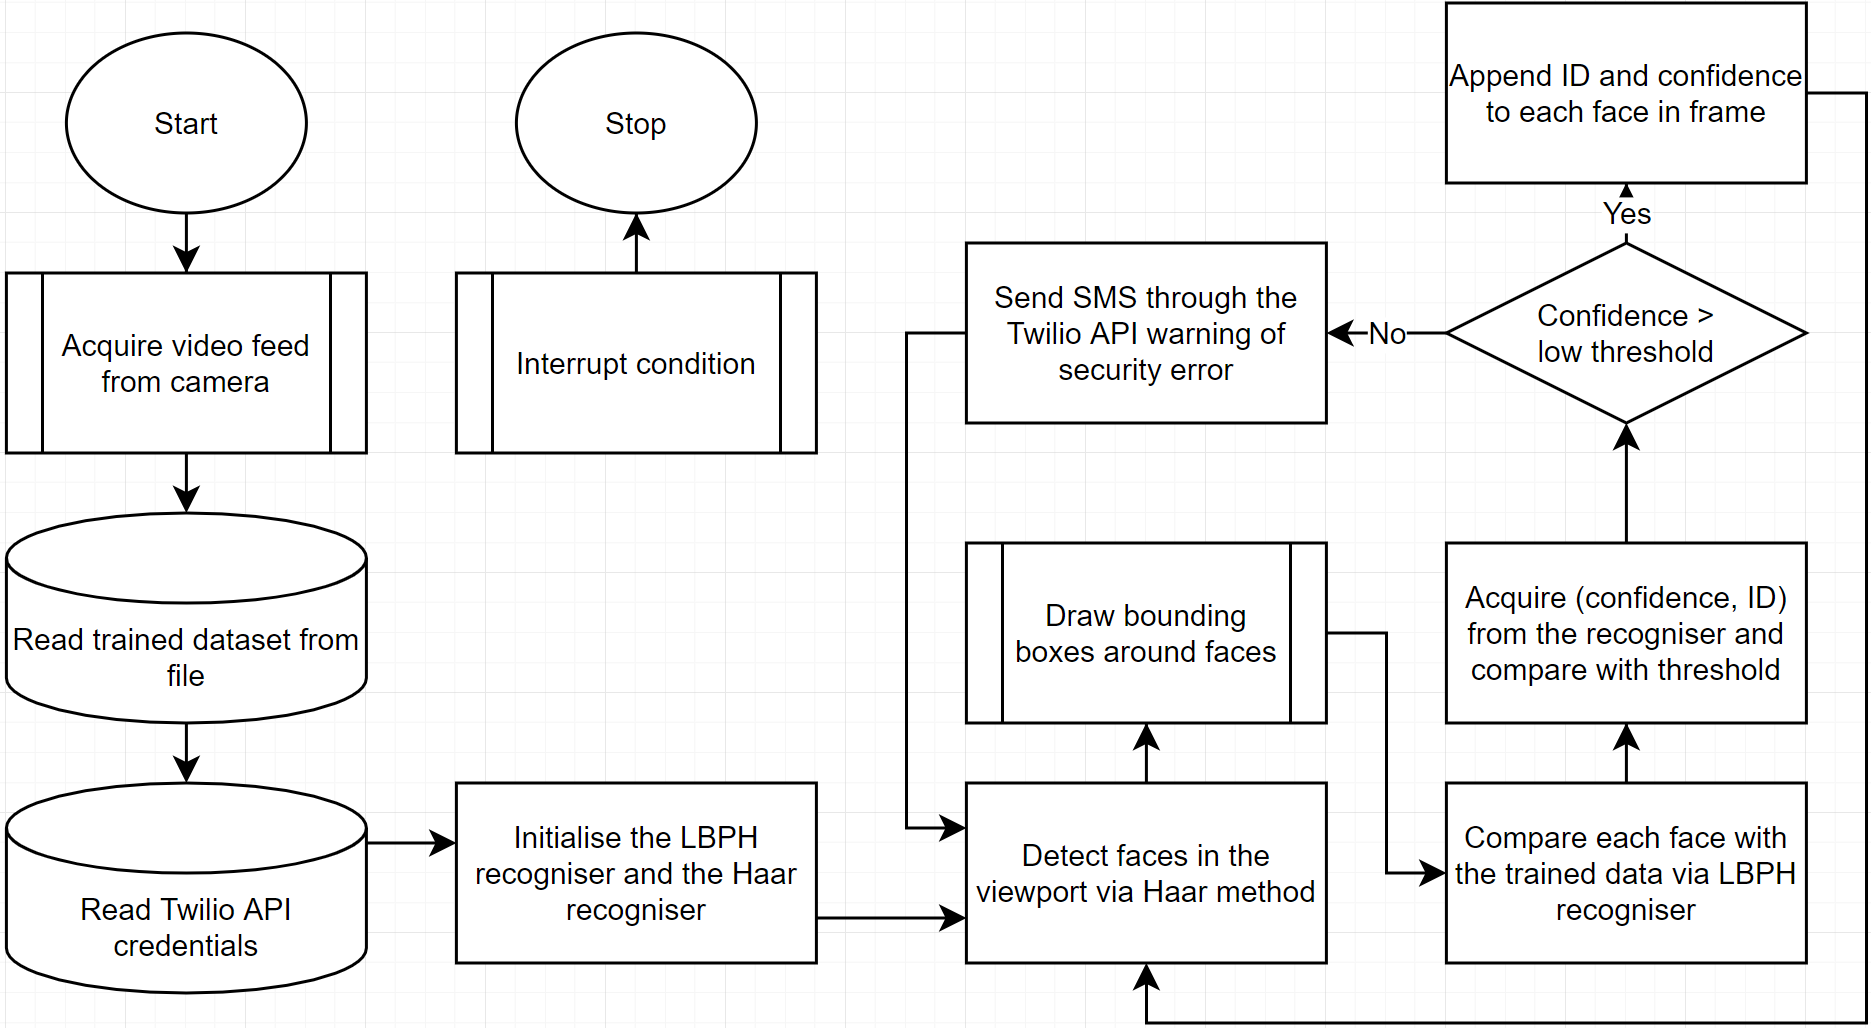
\includegraphics[width=4.7in]{facialRecognitionIdentify.png}
	\caption{A flowchart describing the logic in the identification stage}\label{fig_flowRecognition}
\end{figure}
Despite this, most of this builds upon previous psuedocode as the extra parts are merely additions to the underlying logic from previous sections. Nevertheless, the psuedocode for this part of the solution is as follows.
\begin{lstlisting}
set faceCascade = {path_to_cascade_xml}
set recogniser = {LBPH_recognizer_cv2}
set trainedFile = {path_to_trainer_yaml} 
set stream 	= videoFeed from {device}
set stream{height} = height
set stream{width} = width
set names = names[]
set lowThreshold = {low_threshold}
while True:
	set gray = stream{convert_to_greyscale}
	set faces = detect faces in gray with {parameters}
	for each face in faces:
		{draw_boundingBox} around face
		use recogniser to identify faces
		set (ID, confidence) = {get_prediction} from recogniser
		if confidence > 40:
			set id = names[ID]
		else:
			set id = 'Unknown'
			{send_SMS} with Twilio
		{write_text} of {(confidence, ID)} around each boundingBox
release videoFeed from {device}
\end{lstlisting}
The new additions in this code include the use of the Twilio API to send an SMS to a phone on the condition that there is an intruder, and the use of the \texttt{trainedFile} to recognise faces with the \texttt{\{get\_prediction\}} function (which will be implemented with the \texttt{OpenCV} library).

\subsubsection{The web side of the solution} 
The code designed previously covers the whole facial recognition section of the solution. The next stage is to construct a webpage that allows us to view the results of this facial recognition on any computer connected to the local intranet\footnote{We could also do this over the internet by using port forwarding. Doing this may add security vulnerabilities though as people may be able to hack into the system -- I would rather leave this option disabled as a default}. We must do this by incorporating the previous code into our webserver, which will be constructed with the \texttt{Flask} library in Python. \\\
The top-level flowchart is shown on Figure \ref{fig_webserver} -- this shows the surface level logic of the way in which the webpage will funciton.
\begin{figure}[H]
	\centering
	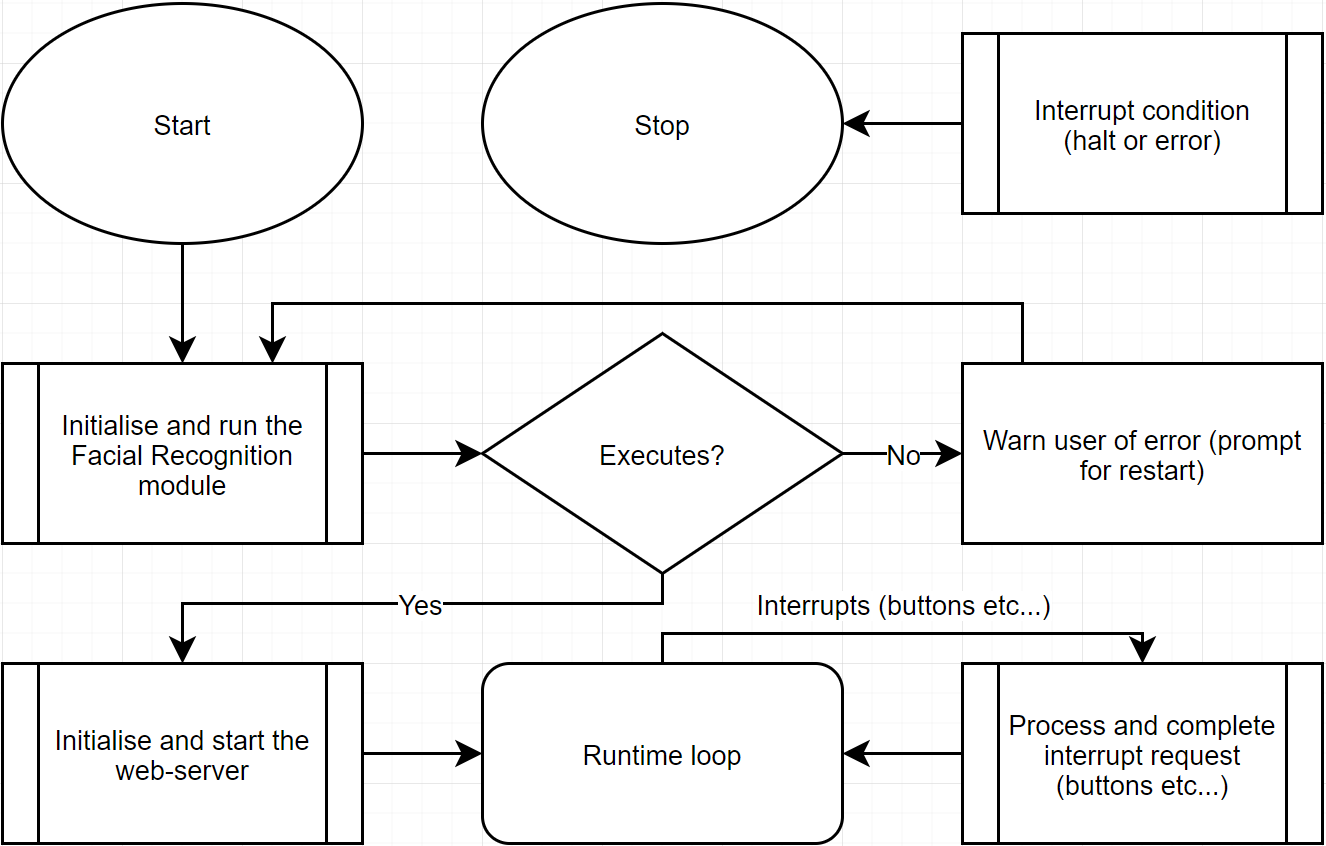
\includegraphics[width=4.8in]{webserverWhole.png}
	\caption{A flowchart showing the top-level logic for the web-server}\label{fig_webserver}
\end{figure}
The sub-process block \texttt{`Initialise and run the Facial Recognition module'} represents all of the previous Facial Recognition code, the rest of the blocks represent the functionality of the webpage. The \texttt{`Runtime loop'} block is there to show that the webpage will be running in a loop, but buttons can still be pressed. If a button is pressed, then the interrupt must be processed before returning back to normality. If the interrupt is a halt or an error then the solution must stop.\\\\
The visual and programmed functions are all designed in the subprocess \texttt{`Initialise and start the web-server'} and this contains most of the content that is of our concern. We can expand the subprocess to its own in order to view the process in more detail. The result is shown on Figure \ref{fig_webserverExpand1}. The main challenge in this portion of the design is working out exactly how the previous (Facial Recognition) code fits into the web-server code.
\begin{figure}[H]
	\centering
	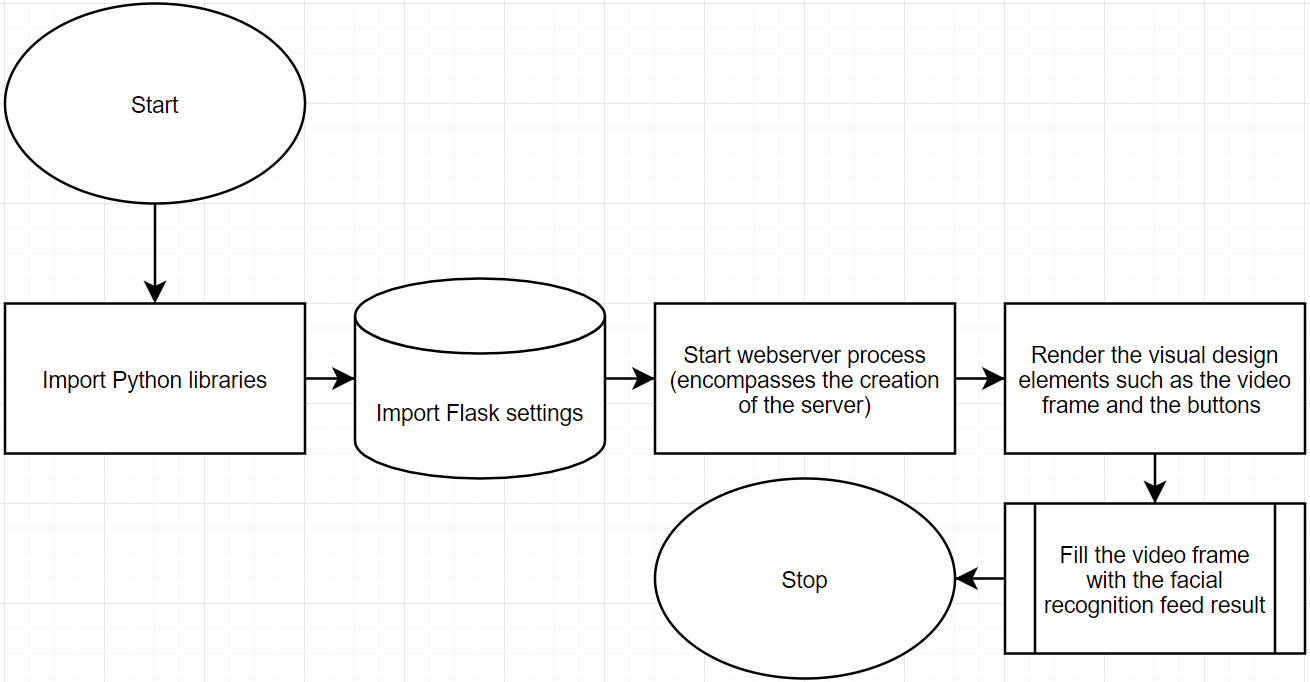
\includegraphics[width=5in]{webserverExtended.png}
	\caption{A flowchart showing the logic in the web-server subprocess from Figure \ref{fig_webserver}}\label{fig_webserverExpand1}
\end{figure}
We can see the logic of the subprocess here; the solution must first load the \texttt{`Flask'} library so that the webserver can be made. The Python implementation for a basic test \texttt{`Flask'} server can written as follows
\begin{lstlisting}
app = Flask(__name__)
@app.route('{URL}')
def tester():
	return "Hello World!"
if __name__ == '__main__':
	app.run()
\end{lstlisting}
For example, setting
\begin{lstlisting}
URL = '\'
\end{lstlisting}
And navigating to \texttt{http://localhost:5000/} (the default port) will return \texttt{`Hello World!'}. Perfect! We now would have a working web-server to put the required elements on. Importing \texttt{Flask} settings as shown in the cylinder flowchart element would allow us to change the default port along with many other settings. This may be useful as we may want to set the options differently than the default. Inside the \texttt{def tester()} is where we would place items such as buttons and the video frame. To do this, I will be importing \texttt{templates} from the \texttt{Flask} library also. This allows us to load a \texttt{HTML} page to show for that particular \texttt{@app.route} (URL) instead of coding it all within the Python code itself. The style of the buttons can then be made and applied with some simple \texttt{CSS} in order to make it clear. \\To add to the success criteria that govern clarity of the webpage, the most common form of colour-blindness affects the ability to perceive the differences in red-green colour spaces\cite{colourBlindness}. Therefore, the buttons must not rely solely on colour as mentioned previously.\\\\
This covers most of the design of the solution. During the iterative development phase it is likely that I will encounter additional nuances and problems that need to be overcome. These will be debugged, the solutions designed and the problems fixed at the stages I encounter them.
		
\newpage
\subsubsection{Identifying key variables, objects, and data structures}

\begin{table}[H]
	\centering
	\rowcolors{3}{tableShade}{white}
	\begin{tabularx}{\textwidth}{llXX}
		\textbf{Variable Name} & \textbf{Data Type} & \textbf{Use of the Variable}                                                                                                                      & \textbf{Validation Needed (If Applicable)}                                                                                              \\ \midrule
		str\_cascadePath       & String             & Stores the path of the Haar Cascade used for recognising a face                                                                                   & No validation needed (Developer)                                                                                                        \\
		obj\_faceCascade       & Object             & The CV2 object that contains the Haar Cascade, called in order to recognise a face                                                                & No validation needed (Developer)                                                                                                        \\
		str\_datasetPath       & String             & The path to the dataset that stores the faces                                                                                                     & No validation needed (Developer)                                                                                                        \\
		obj\_stream            & Object             & The camera, as an object. This is separate from the video feed from the camera                                                                    & No validation needed (Developer)                                                                                                        \\
		obj\_videoFeed         & Object             & The images that come trough obj\_stream, not the camera itself but the resulting images that we need to work with                                 & No validation needed (Developer)                                                                                                        \\
		str\_recogniserPath    & String             & The path to the trained file that contains the instructions for recognising faces                                                                 & No validation needed (Developer)                                                                                                        \\
		obj\_recogniser        & Object             & The CV2 object that is called to identify a particular face, uses the trained file in str\_recogniserPath                                         & No validation needed (Developer)                                                                                                        \\
		int\_id                & Integer            & Keeps track of which set of images belongs to which person. This can be seen as a UID as it eliminates the problems with duplicate names          & No validation except for when the user inputs an ID for dataset collection. Validation is that it must be an integer \\
		obj\_font              & Object             & The font used when writing text with CV2                                                                                                          & No validation needed (Developer)                                                                                                        \\
		real\_minWidth         & Real (Float)       & The minimum dimensions for the Haar cascade when trying to scale the face to compare. Useful for eliminating false positives of very small images & No validation needed (Developer)                                                                                                        \\
		real\_minHeight        & Real (Float)       & The minimum dimensions for the Haar cascade when trying to scale the face to compare. Useful for eliminating false positives of very small images & No validation needed (Developer)                                                                                                        \\
		arr\_names             & Array              & The list of names, this can be loaded from a file such as a CSV file that is maintained by Python                                                 & No validation needed (Developer)                                                                                                        \\
		real\_confidence       & Real (Float)               & This is the measure of confidence received from the CV2 recogniser                                                                                & No validation needed (Developer)                                                                                                        \\
		&                    &                                                                                                                                                   & No validation needed (Developer)                                                                                                        \\[0.5cm] 
		&                    &                                                                                                                                                   & No validation needed (Developer)                                                                                                        \\ \hline
	\end{tabularx}
	\caption{A table identifying the key variables, objects, and data structures with justification}
	\label{tab_keyItems}
\end{table}
In the table above, we can see the switch case and Hungarian notation at work -- these provide clarity to each and every variable used in the program. This, along with comments along the code, will make clear to others what each section of the code does.









\newpage
\subsection{Describing the testing methodology}
\subsubsection{Testing the setup of the device}
\begin{table}[H]
	\centering
	\rowcolors{3}{tableShade}{white}
	\begin{tabularx}{\textwidth}{lXlXX}
		\textbf{Test} & \textbf{Test Data}                                                        & \textbf{Test Type} & \textbf{Test Reason}                                                                                                               & \textbf{Expected Outcome}                                      \\ \midrule
		1             & Ensure that the Pi receives power and can boot into the OS on the SD card & Normal             & The soution will be deployed on a raspberry Pi, the Pi therefore needs to be working                                               & The Pi should boot into the OS on the SD card                  \\
		2             & Ensure that the SSH connection works                                      & Normal             & We will be accessing the Pi through SSH as that allows for more usability (less cables due to headless setup)                      & SSH works correctly and the Pi can connect to PC through PuTTY \\
		3             & Ensure that the Pi VNC server works correctly and that the PC can connect & Normal             & VNC allows us to see the desktop environment from the Pi on our PC -- once again for usability reasons                             & The VNC sever works correctly and we can connect from our PC   \\
		4             & Ensure that Python is updated to the latest version                       & Normal             & This ensures the highest compatibility with bug fixes etc                                                                          & The Python installation is of the latest version               \\
		5             & Ensure that OpenCV is installed and is of the latest version              & Normal             & The core of the facial recognition part of the solution uses OpenCV, we must therefore have the latest and most compatible version & The latest version of OpenCV is installed (Pip)                \\
		8             &                                                                           &                    &                                                                                                                                    &                                                                \\ \bottomrule
	\end{tabularx}
	\caption{A table showing the tests performed on the device, with justification}
	\label{tab_testingDesignDevice}
\end{table}
Once these tests are complete, we can say that the device is ready to start being used to develop the solution on --  all the necessary components and dependencies are now there. The nexct stage is now working out a testing frame for the solution. This is a much larger task due to the scale of the solution and the immense amount of work needed to process and perform each test on each component


\subsubsection{Testing the solution}
\begin{table}[H]
	\centering
	\rowcolors{3}{tableShade}{white}
	\begin{tabularx}{\textwidth}{lXlXX}
		\multicolumn{1}{l}{\textbf{\begin{tabular}[c]{@{}l@{}}
			 Test  \\
			Number
		\end{tabular}}} & \textbf{Test Data}            & \textbf{Test Type} & \textbf{Test Reason}           & \textbf{Expected Outcome}      \\ \midrule
		1                                                                                   & bla bla this is the test data & Normal             & To check to make sure it works & To check to make sure it works \\
		2                                                                                   &                               &                    &                                &                                \\
		3                                                                                   &                               &                    &                                &                                \\
		4                                                                                   &                               &                    &                                &                                \\
		5                                                                                   &                               &                    &                                &                                \\
		6                                                                                   &                               &                    &                                &                                \\
		7                                                                                   &                               &                    &                                &                                \\
		8                                                                                   &                               &                    &                                &                                \\
		9                                                                                   &                               &                    &                                &                                \\
		10                                                                                  &                               &                    &                                &                                \\
		11                                                                                  &                               &                    &                                &                                \\
		12                                                                                  &                               &                    &                                &                                \\
		13                                                                                  &                               &                    &                                &                                \\
		14                                                                                  &                               &                    &                                &                                \\ \bottomrule
	\end{tabularx}
	\caption{A table showing the tests performed on the solution, with justification}
	\label{tab_testingDesignSolution}
\end{table}
Once this is complete and the solution has been finished (one stage from production/deployment) we can then move on to the final testing frame. This ensures one last time that the components work and most importantly, ensures that they work well together to form the final product.

\subsubsection{Final Testing}
\begin{table}[H]
	\centering
	\rowcolors{3}{tableShade}{white}
	\begin{tabularx}{\textwidth}{lXlXX}
		\multicolumn{1}{l}{\textbf{\begin{tabular}[c]{@{}l@{}}
					Test  \\
					Number
		\end{tabular}}} & \textbf{Test Data}            & \textbf{Test Type} & \textbf{Test Reason}           & \textbf{Expected Outcome}      \\ \midrule
		1                                                                                   & bla bla this is the test data & Normal             & To check to make sure it works & To check to make sure it works \\
		2                                                                                   &                               &                    &                                &                                \\
		3                                                                                   &                               &                    &                                &                                \\
		4                                                                                   &                               &                    &                                &                                \\
		5                                                                                   &                               &                    &                                &                                \\
		6                                                                                   &                               &                    &                                &                                \\
		7                                                                                   &                               &                    &                                &                                \\
		8                                                                                   &                               &                    &                                &                                \\
		9                                                                                   &                               &                    &                                &                                \\
		10                                                                                  &                               &                    &                                &                                \\
		11                                                                                  &                               &                    &                                &                                \\
		12                                                                                  &                               &                    &                                &                                \\
		13                                                                                  &                               &                    &                                &                                \\
		14                                                                                  &                               &                    &                                &                                \\ \bottomrule
	\end{tabularx}
	\caption{A table showing the \textbf{final} tests performed on the solution, with justification}
	\label{tab_testingDesignSolutionFinal}
\end{table}


















\newpage
\section{The Iterative Development Process}
We can now begin the iterative development process; using the success criteria and the testing frames we made in the previous section, we can begin to write the code that will build the solution we planned. It is important that the code is tested along the way to ensure that each `block' of code works before pushing them all together to create a final solution.\\\\
In this section, each subsection is a different code `block' that will be independently tested as per the testing frame. As well as the success criteria, the code must adhere to the points specified in the success criteria we constructed before in order to be consistent with what we want from our solution. Each subsection will be evaluated in order to accurately assess how it performs in comparison to our needs.\\\\
Performing the production of code in this way allows us to ensure any errors are not carried through late into the development process. If an error occurs early in the construction of the solution, we will find out before moving on to other sections of code. This is important as if there are any errors, we will not have to debug multiple errors at any one time (hopefully).\\\\
Whilst the code will be modular, the way in which we decide which area to code is fairly linear due to many parts of the solution relying on previous parts. The parts that will be coded first will be something in the order of;
\begin{enumerate}
	\item Setting up the Pi
	\item Coding the facial development area of the solution, use developer testing
	\item Create the webpage and add all the required elements (these can be placeholders)
	\item Integrate the facial recognition portion into the webpage that we created
	\item Final testing
\end{enumerate}
As mentioned previously, testing will occur in each stage (independently of other stages).\\\\
\begin{figure}[H]
	\centering
	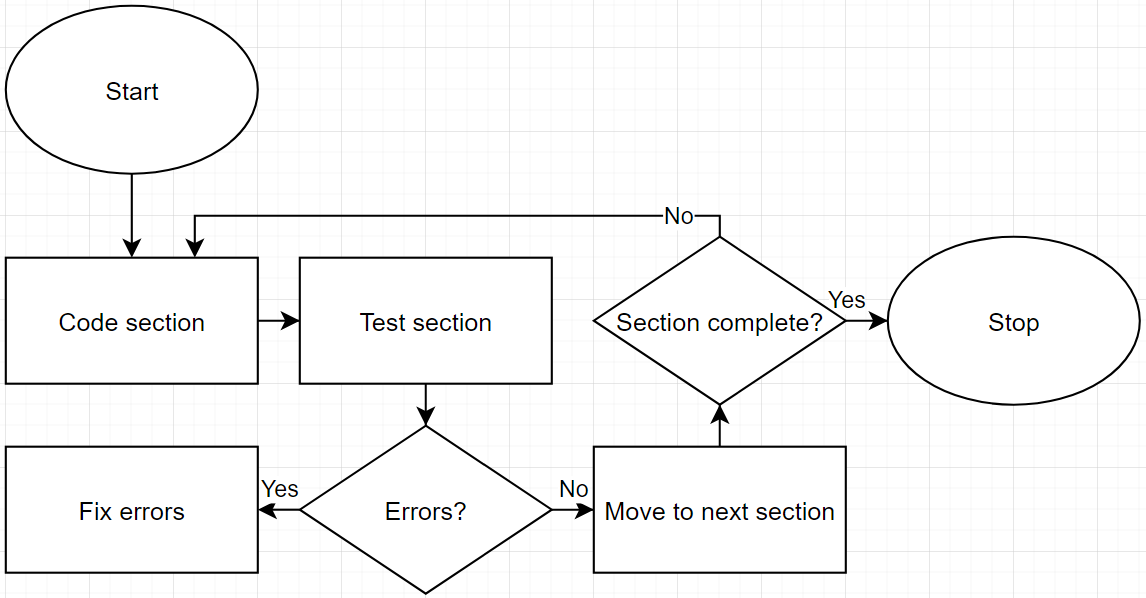
\includegraphics[width=6in]{flowTesting.png}
	\caption{A flowchart showing how the testing logic links to our development}\label{fig_flowTesting}
\end{figure}
On Figure \ref{fig_flowTesting}, we can see how we will perform testing at each stage. With this in mind, we can now begin the development process.











\newpage
\subsection{Setting up the Raspberry Pi}
We begin setting up the hardware for our Raspberry Pi 3B.
\begin{figure}[H]
	\centering
	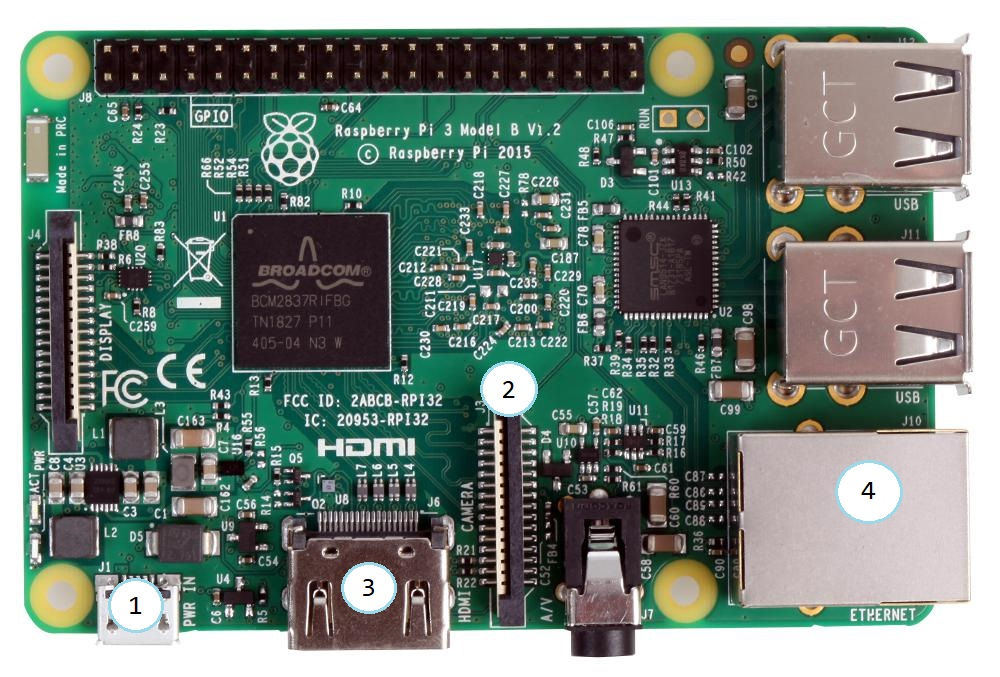
\includegraphics[width=4in]{raspberryPi.jpg}
	\caption{A picture showing the connections available on the Pi 3B}\label{fig_raspberryPi}
\end{figure}
We can see the connections available to us on Figure \ref{fig_raspberryPi}, the list below tells us the function of each part.
\begin{enumerate}
	\setlength{\itemsep}{4pt}
	\setlength{\parskip}{0pt}
	\item Micro USB power input @ 5V \& 4A
	\begin{itemize}
		\item This powers the Pi, and we will be adding a power supply here in order to use the Pi. There is a GPIO add on that allows us to use PoE (which will reduce the total amount of cables), however I will be sticking to the basic way of powering the Pi
	\end{itemize}
	\item Camera ribbon cable connector
	\begin{itemize}
		\item The NoIR camera connects to other devices via a ribbon cable. The slot on the Pi here is where the cable wil be connected to
	\end{itemize}
	\item HDMI output
	\begin{itemize}
		\item This is where we would be plugging the HDMI output cable to connect to a monitor. However, we will be using SSH right from the start so this cable is not needed
	\end{itemize} 
	\item Ethernet connector
	\begin{itemize}
		\item This connector is used to allow the Raspberry Pi to connect to the internet. In deployment, the internal Wi-Fi will be used. Despite this, I will be using Ethernet during development as it is more reliable
	\end{itemize}
\end{enumerate}
Both the Raspberry Pi and the NoIR camera are reasonably delicate, and neither are waterproof. As a result, both will need to be put in a waterproof housing before they can be sold as a product. During early development. Even with this in mind, I will be keeping both components out of their cases in the early phases of development so that I have more control over the hardware (just in case).\\\\
Once all the connections have been made, the next step is to write an operating system image on to an SD card. I will be using Rufus\cite{Rufus} for this task -- freeware that allows us to write an image in \texttt{.img} format to an SD card.\\\\
I will be using Raspberry Pi OS\cite{raspberryPi} (previously called Raspbian OS) on my Pi, this is a good all around operating system due to its low resource footprint. In addition, it comes with out-of-the-box support for the Pi NoIR camera. After using Rufus to flash the SD card with the image, the SD can then be inserted into the slot (not visible on Figure \ref{fig_raspberryPi} due to the fact it is on the underside of the Pi) and the Pi can be powered on.
An important thing to note is that I needed to add a file with the name \texttt{ssh} with no extension in the \texttt{boot} partition of the SD card. This tells the Pi to enable the SSH server by default on boot without having to connect peripherals to the Pi directly. With this, I can then SSH into the Pi through PuTTY, where I am greeted with the screen shown in Figure \ref{fig_raspberryPiBoot}
\begin{figure}[H]
	\centering
	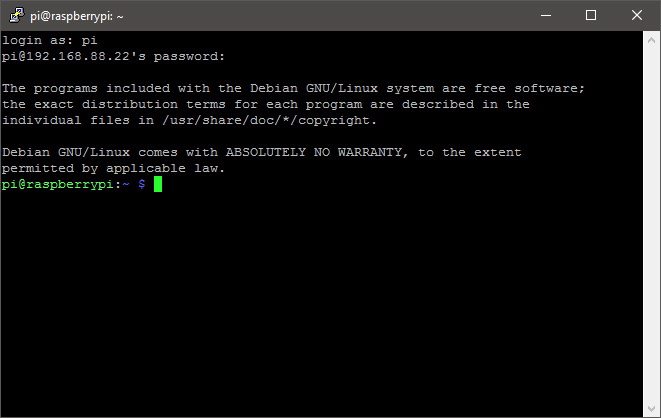
\includegraphics[width=4in]{raspberryPiBoot.png}
	\caption{The login screen for the Pi terminal, shown on the PuTTY terminal}\label{fig_raspberryPiBoot}
\end{figure}
This section covers Criterion 1($\alpha$) as we now have an SSH terminal (and therefore access to the Raspberry Pi). The next step  is to enable the VNC server (if not enabled by default). The reason that I have not only enabled the VNC server is so in the case of an error with VNC, we can always (attempt) to fallback to SSH which should allow us to fix the VNC server. \\\\
For Criterion 2($\alpha$), we must enable the VNC server if it is not enabled already. We can verify if it is enabled by opening VNC viewer on the desktop and attempting to connect to the IP address of the Pi with the default user credentials. Doing this results in the desktop screen of the Pi being shown -- voilà! The VNC server is enabled by default so we do not need to worry about enabling it, if anything happens, we can always revert back to using SSH in a worst case scenario. The desktop is shown on Figure \ref{fig_vncDesktop} and by checking in the display settings, we can verify as per Criterion 2($\alpha$) that the resolution is at least 768p. Importantly, there is no perceivable desktop stutter apart from when performing intense operations on the CPU; a result of heavy mathematical operations being performed by the arithmetic logic unit and these operations taking most of the CPU time.\\\\
The next stage of preparing the device will be setting up the NoIR camera for use with the Pi so that we can then use the video feed for later parts of the development. To do this, the Pi is turned off before connecting the ribbon cable from the camera to the appropriate connector as described previously in Figure \ref{fig_raspberryPi}. The Pi can then be powered on and the Pi settings command, \texttt{raspi-config}, can be used in the terminal to access the list of settings available for us to tweak on our Pi. The settings for the camera can then be toggled in order to enable the camera add-in module.\\
Later, to verify that the camera works, we can use the \texttt{raspistill} command to take a still photo with the camera which is saved in the current working directory of the terminal where the command was called. If there is a photo that resembles what the camera should see then we can move on with this. As per criterion 3($ \alpha $), the only thing that needs to happen at this stage is that the command takes and saves a photo, and the photo is recognisable from the current position of the camera.\\\\
For Criterion 4($ \alpha $), we must change the swap size on the Pi. This is due to the fact that the default swapsize is quite low. As a result, memory intensive tasks may cause the system to run out of memory and then hang or crash -- this is a scenario that must be avoided. To combat this, the swapsize can be changed with the following sequence of commands;
\begin{lstlisting}
sudo dphys-swapfile swapoff		# turns the swapfile off
sudo nano /etc/dphys-swapfile	# this is used to open and edit the file
sudo dphys-swapfile swapon		# turns the swapfile on
free -m							# returns an output resembling the below

----------------------------------------------------------------------------
					total	used	free	shared	buffers	cached
Mem:          		435     56		379		0		3       16
-/+ buffers/cache: 	35      399		----	----	----	----
Swap:         		1023    0     	1023	----	----	----
----------------------------------------------------------------------------
\end{lstlisting}
After we open up the file with \texttt{nano}, we must change the line \texttt{CONF\_SWAPSIZE=100} to \texttt{CONF\_SWAPSIZE=1024}
The \texttt{free -m} command gives us a rundown of memory usage on our system. If the total swapdisk size is what we set the new size as, then the swapdisk size change worked as needed in Criterion 4($ \alpha $)\\\\
Criterion 5($ \alpha $) governs what software we need on our system. Most importantly for the solution, we need a relatively new version of Python 3.x.x which is also compatible with OpenCV. The latest version of Python on the website is listed as XXXXXXXXXXX and we need at least XXXXXXXXXXXXX for OpenCV to work. \\
As a precautionary measure, I ran the following commands to ensure everything else on the system was up to date. These commands should also update Python as it is pre-installed on the system.
\begin{lstlisting}
sudo apt-get update				# to update the package information from registered sources
sudo apt-get upgrade			# to upgrade packages to their new release (if it exists)
\end{lstlisting}
This ties in nicely with Criterion 5($ \alpha $) as to move on, we now need to install OpenCV. This can be done very easily  with the command \texttt{pip install opencv-python}. This installs the OpenCV package into our installation of Python automatically without the need to compile everything.\\\\
With the device set-up, we can now move on to testing that is, infact, set-up correctly. We can do this by comparing the expected outcome of the corresponding testing harness table made previously, to the actual results of testing.
\begin{table}[H]
	\centering
	\rowcolors{3}{tableShade}{white}
	\begin{tabularx}{\textwidth}{lXXXl}
		\textbf{Test} & \textbf{Test Data}                                                                               & \textbf{Expected Outcome}                                                 & \textbf{Actual Outcome}                                                                       & \textbf{Passed?} \\ \midrule
		1             & Adding power and watching for the LED lights on the board to indicate a successful boot sequence & The Pi should boot into the OS on the SD card                             & The Pi boots into the OS loaded on to the SD card. This is verifiable by SSH in the next test & YES              \\
		2             & Attempting to connect to the Pi via SSH with its IP address and default credentials            & We should get a terminal on our desktop which allows us to control the Pi & We are given a terminal and are free do perform any commands as you would on the Pi itself    & YES              \\
		3             & Attempt to connect to VNC server via IP address and default credentials & The VNC sever works correctly and we can connect from our PC, showing a desktop environment
& The client connects via VNC and we are successful in having a desktop environment & YES \\
		4             & Running \texttt{Python} in the terminal to aquire the version number & The version matches a release within the last 6 months & The version was XXXXXXXXXX, which is XXXXX months old & YES \\
		5             & Using the command \texttt{pip freeze} to view currently installed packages and their version & The version is less than 3 months old & The version was less than 3 months old & YES \\ \bottomrule
	\end{tabularx}
	\caption{A table showing the tests performed on the device setup, the result of the test, and success/failure}
	\label{tab_deviceSetupTesting}
\end{table}
As all the tests needed for this section of construction have passed and that the success criteria governing the creation of this section has been adhered to, we can now move on to the next section of construction.


\newpage
\subsection{Getting a working video feed with OpenCV}
For the next sections to work, we must generate some code that allows us to get a working image feed in Python. As we are using VNC and can see the desktop environment, it is sufficient to output the feed captured by OpenCV to a graphical window for now. Later on in the development after we move to the webpage, this will become deprecated and will be removed.

I began with the following code in Python, comments are attached to the side and underneath certain lines for explanation.
\begin{lstlisting}[language=Python]
import cv2 
# import the OpenCV library used for facial recognition into our code, we can then call all functions in this library
str_cascadePath =  'Cascades/haarcascade_frontalface_default.xml'
# this file was taken directly from the OpenCV GitHub repo
obj_faceCascade = cv2.CascadeClassifier(str_cascadePath) 
# create a classifier object that is used to identify faces, we will be using the cascade that str_cascadePath points to
obj_stream = cv2.VideoCapture(1) 
# access the NoIR by creating an OpenCV object that uses the camera
obj_stream.set(3,800) 
obj_stream.set(4,600)
# set camera width and height (800x600)
while True: 
# this is a basic runtime loop, i am to change this when i add the web interface to call this as a function
	working, obj_videoFeed = stream.read() 
	# 
	obj_videoFeed = cv2.flip(obj_videoFeed, -1) 
	# my setup needs the camera to be flipped due to its placement
	obj_videoFeedGray = cv2.cvtColor(obj_videoFeed, cv2.COLOR_BGR2GRAY) 
	# create a grayscale version of the frames captured using the OpenCV conversion
	faces = faceCascade.detectMultiScale(gray, scaleFactor=1.2, minNeighbors=5, minSize=(30, 30)) 
	# calls the function to detect faces using the Haar Cascade, applied to the gray image
	for (x,y,w,h) in faces: 
		# for each face...
		cv2.rectangle(imgout,(x,y),(x+w,y+h),(0,0,0), 1) 
		# draw a black rectangle of thickness 1 as a bounding box around the face
		img_gray = obj_videoFeedGray[y:y+h, x:x+w] 
		# creates images of the face detected in greyscale and in color
		img_color = obj_videoFeed[y:y+h, x:x+w] 
		# ive added these now to be used later when saving photos of unknown people, just for testing at the moment
	cv2.imshow('Input feed', obj_videoFeed) 
	# creates a window and streams the input from the camera from the variable imgout
	key_k = cv2.waitKey(10) & 0xff 
	# continually updates the image as long as ESC isnt pressed
	if key_k == 27:
		# if ESC pressed
		break 
		# break on ESC
stream.release() 
# free the camera, keep the hardware and software (mainly memory) tidy, this prevents errors with the camera being in-use whilst we try to run the code
cv2.destroyAllWindows() 
# destroy the image window
\end{lstlisting}
When this code is ran, the following window pops up which shows the result of Haar detection.






\newpage
\section{Evaluation}












\newpage
\subsection{Testing the product against our final criteria}











\newpage
\subsection{Sucess of the solution}











\newpage
\subsection{Describing the final product}












\newpage
\subsection{Problems I encountered and what I would do in the future}











\newpage
\addcontentsline{toc}{section}{Bibliography}
\bibliography{biblio}
\end{document}
%
%\begin{table}[H]
%	\centering
%	\rowcolors{3}{tableShade}{white}
%	\begin{tabularx}{\textwidth}{lXXXl}
%		Test & \textbf{Test Data} & Expected Outcome & Actual Outcome & Passed? \\ \midrule
%		1    &                    &                  &                &         \\
%		14   &                    &                  &                &         \\ \bottomrule
%	\end{tabularx}
%	\caption{A table showing the tests performed on the solution, with justification}
%	\label{tab_testingDesignSolution}
%\end{table}